\problemname{Museum Guard Shift}

A museum has $N$ rooms connected by corridors. The corridors form a tree, so there is exactly one simple path between any two rooms.

A night guard starts in room $S$ at time $0$. Exactly $K$ rooms contain alarms.

To handle an alarm in room $u$, the guard must first travel to $u$, then spend $a_u$ units of time opening the security panel in that room. The guard handles the alarm in room $u$ successfully only if this process finishes no later than time $d_u$.

The guard may pass through rooms and corridors any number of times. Traversing a corridor of length $w$ takes $w$ units of time.

Determine the minimum total time needed to handle all alarms, or report that it is impossible.

\section*{Input}

The first line contains three integers: $N$, $K$, $S$ ($1 \le N \le 200\,000$, $0 \le K \le 18$, $1 \le S \le N$).

The next $N-1$ lines each contain three integers $u$, $v$, and $w$, meaning there is a corridor between rooms $u$ and $v$ with traversal time $w$ ($1 \le u,v \le N$, $1 \le w \le 10^9$).

The next $K$ lines each contain three integers $r_i$, $a_i$, and $d_i$, meaning room $r_i$ is alarmed, handling its alarm takes $a_i$ time, and it must be completed by time $d_i$ ($1 \le r_i \le N$, $1 \le a_i \le 10^9$, $1 \le d_i \le 10^{15}$).

\section*{Output}

Print a single line containing either the minimum total time required to handle all alarms, or \texttt{IMPOSSIBLE} if no valid schedule exists.

\subsection*{Sample tree}

Both sample inputs share the tree below (blue node = start room, red nodes = alarmed rooms).

\begin{center}
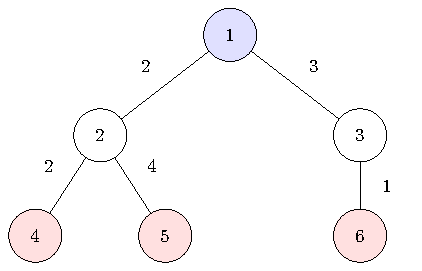
\includegraphics[width=0.45\textwidth]{tree_diagram}
\end{center}

\subsection*{Explanation of sample 1}
One optimal order is:
\begin{itemize}
    \item go to room $4$: travel $4$, open for $1$, finish at time $5$
    \item go to room $6$: travel $8$, open for $2$, finish at time $15$
    \item go to room $5$: travel $10$, open for $1$, finish at time $26$
\end{itemize}
All deadlines are met, so the answer is $26$.

\subsection*{Explanation of sample 2}
The earliest possible time to finish room $4$ is $5$, but its deadline is $4$, so no valid route exists.
